\chapter{Datasets}
\label{cha:datasets}

In the previous chapter, we presented the fundamentals of highly overlapped audio signals.
To study these signals in a reproducible manner, suitable data is of paramount importance since many methods rely on audio datasets for development and evaluation.
However, suitable audio material is not publicly available, in the case of music, often because of restrictive copyright laws. 
Therefore, in the past, many academic endeavors were focussed on assembling such precious data. 
In fact, in the audio community, datasets contributions now are essential to  accelerate many research directions.
\par
In the following sections, we present three datasets which we helped creating.
Each of the three datasets is released in public domain and aim to fill specific needs and are used in subsequent experiments throughout this thesis.

\section{Unison Mixtures}
\label{sec:unison_dataset}

\marginpar{
  Parts of this this section were previously published in~\cite{stoter14}.
}

In speech, it is common to mix clean speech and noise~\cite{varga93} or different clean speech signals such as~\cite{garofolo93} to generate mixtures.
By contrast, the conversational aspect of human-to-human communication is lost.
Compared to speech, musical content usually does share familiar orchestration, can hardly be superimposed randomly and the summing of isolated random notes from musical instrument databases does not reflect musical performances.
On the positive side, there are use-cases for single note datasets such as for evaluation of fundamental frequency estimation algorithms or the detection of instruments.
Furthermore, single note datasets allow using the data to synthesize musical score as long as the recordings have enough variance of expressions.
It also allows to quickly generate a large number of mixtures using randomly permuted mixtures, fostering applications in machine learning.

As an exception compared to other music scenarios, when all instruments play~\emph{in unison}, single note datasets are appropriate to approximate real mixtures:

\begin{itemize}
  \item A random summation of multiple instruments playing the same note does not necessarily differ from realistic unison mixture.
  \item When notes are played with vibrato, having access to the individual modulation patterns can help to study the influence of modulations systematically.
  \item Unison mixtures are part of many classical compositions, to extend the timbre of a note.
\end{itemize}

\par
One way to assemble a dataset is to create random mixtures of single notes compiled from existing datasets such as the \emph{Univ. of Iowa Musical Instrument Sample Database}\footnote{\url{http://theremin.music.uiowa.edu/index.htm}}.
However, to better study the influence of vibrato we require extended control over certain parameters such as note duration, vibrato duration, exact fundamental frequency, vibrato rate, vibrato extend, reproducibility, loudness or expression.
\par
As mentioned in previous chapter, vibrato techniques vary across instruments. 
Instruments such as violin and tenor sax are known for its distinct frequency modulations~\cite{gilbert05}.
Other instruments such as the English horn and the flute are more close to amplitude modulations.
\par
We, therefore, generated the notes using a software sampler\footnote{\textsc{Vienna Symphonic Library}: \url{https://vsl.co.at}} which allows us to control the parameters such as the vibrato.
All our test stimuli have a duration of three seconds.
Items were equalized in loudness by using an iterative calculation of the loudness algorithm of the time-varying Zwicker model~\cite{zwicker13}. 
We used an implementation released in~\cite{genesis12}. 
\par
We rendered 29 notes of C4, resulting in 841 unique unison instrument mixtures per pitch class.
An excerpt of the instruments is listed in Table~\ref{tab:testset}.
The dataset is available from~\cite{oss_unison}.

\begin{table}
\begin{center}
\footnotesize
\begin{tabular}{ l l l}
  \toprule
  Instrument & Vibrato &  MIDI \# \\
  \midrule
  Violin & yes & 40 \\
  Viola & yes & 41 \\
  Violon Cello & yes & 42 \\
  Trumpet & no & 56 \\
  Trombone & no & 57\\
  Horn & no & 60  \\
  Bariton Sax & yes & 67 \\
  Oboe & no & 68\\
  Clarinet & no & 71\\
  Flute & yes & 73\\
  \bottomrule
\end{tabular}
\end{center}
\caption{Selected Instruments from the \emph{Unison Source Separation Dataset}~\cite{oss_unison} as used in~\cite{stoeter14, stoeter16}.}
\label{tab:testset}
\end{table}

To evaluate the level of overlap, we created a small experiment where we computed the average W-disjoint orthogonality \(WDO\) metric for 1000 random combinations of mixtures for different separation scenarios.
It turned out that for two sources, in speech we observe \(WDO=0.9\) and for the vocal/accompaniment scenario \(WDO=0.87\). 
These numbers are surprisingly similar even though both scenarios are so fundamentally different.
In the case of two instruments playing in unison, the average WDO is \(0.65\), indicating that a good separation in the time-frequency domain is more challenging, thus making the dataset a useful addition compared to existing scenarios.


% \begin{figure}
% \begin{tikzpicture}
%     \definecolor{color1}{rgb}{0.298039215686275,0.447058823529412,0.690196078431373}
%     \definecolor{color0}{rgb}{0.917647058823529,0.917647058823529,0.949019607843137}
%     \definecolor{color4}{rgb}{0.768627450980392,0.305882352941176,0.32156862745098}
%     \definecolor{color2}{rgb}{0.333333333333333,0.658823529411765,0.407843137254902}
%     \definecolor{color5}{rgb}{0.8,0.725490196078431,0.454901960784314}
%     \definecolor{color3}{rgb}{0.505882352941176,0.447058823529412,0.698039215686274}
%     \begin{axis}[
%       xlabel=Number of Sources,
%       ylabel=Separability/WDO,
%     ]
%     % speakers
%     \addplot[color=color0,mark=x, line width=1pt] coordinates {
%         (2,0.9)
%         (3,0.79)
%         (4,0.69)
%         (5,0.6)
%         (6,0.536)
%         (7,0.462)
%         (8,0.4197)
%         (9,0.352199)
%         (10,0.32)
%   };
%   % single note
%       \addplot[color=color1,mark=x] coordinates {
%         (2,0.928)
%         (3,0.864)
%         (4,0.8)
%         (5,0.77)
%         (6,0.682)
%         (7,0.637)
%         (8,0.592)
%         (9,0.5647)
%         (10,0.5434)
%   };
%   % unison
%     \addplot[color=color2,mark=x] coordinates {
%         (2,0.626)
%         (3,0.32)
%         (4,0.2)
%         (5,0.13)
%         (6,0.083)
%         (7,0.038)
%         (8,0.025)
%         (9,0.017)
%         (10,0.01)
%     };
%     \end{axis}
% \end{tikzpicture}
% \end{figure}

\section{High Resolution Vibrato Recordings}%
\label{sec:muserc}

\marginpar{
  Parts of this this section were previously published in~\cite{stoeter15acm}.
}

Fundamental frequency \(F_0\) estimation of a signal is a common task in audio signal processing with many applications. 
If the $F_0$ varies over time, the complexity increases, and it is also more difficult to provide ground truth data for evaluation.

\begin{figure}[h]
  \centering
  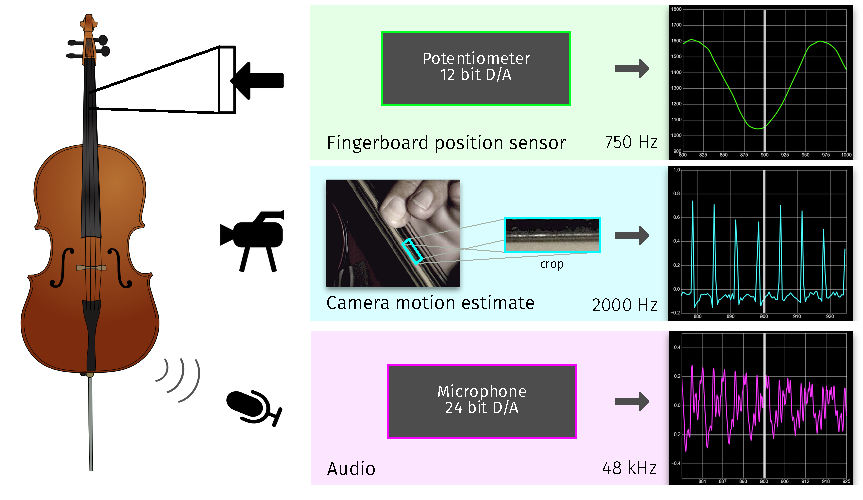
\includegraphics[width=\textwidth]{Chapters/04_Data/figures/teaser.pdf}
  \caption{Overview of the multi-modal data recorded for the proposed dataset.}
\label{fig:teaser_hdf0}
\end{figure}

% from stoter acm
For speech signals, an EGG device (also known as laryngograph) captures the excitation of the human vocal tract. 
This signal is then processed by an $F_0$ estimator to generate the ground truth. 
Such a method is accepted in published research because the EGG signal is considered to be easier to process than speech. 
The retrieved $F_0$-trajectory based on the EGG signal is easier to process and the generated annotations are considered as a good ground truth~\cite{pirker11, babacan13}.
Motivated by this, we proposed a new data set for musical instruments where we recorded a violin cello with extra sensors on the fretboard in addition to audio and video.
We made use of multiple sensors to capture the most relevant processes involved in creating time-varying output signals as depicted in Figure~\ref{fig:teaser_hdf0}.
We included sensor recordings capturing the finger position on the fingerboard which is converted into an instantaneous frequency estimate.
We also included high-speed video camera data to capture excitations from the string at 2000 fps.
Recording video data was inspired by the work of Davis et.\ al.\ in~\cite{Davis2014VisualMic} presenting a ``visual microphone'' which is able to observe sound solely with a camera, pointing to objects in the sound field. 
\par
In the proposed dataset we chose the violin cello for the following reasons: (1) vibrato is used as a common style for expression, (2) there is an observable physical relationship between frequency modulation and vibrato, and (3) the instrument is large enough to embed sensors to capture the vibrato. The properties of the cello are studied by research in acoustics~\cite{woodhouse04, woodhouse99}.
\par
To capture significant aspects of the cello while being played by a musician, we focus on three main observations: (1) Excitation caused by the moving bow; (2) the vibrating string, and (3) the finger, controlling the string length by rolling it on the fingerboard.
The main focus of the recordings is to analyze vibrato playing style. Since it is common that vibrato characteristics differ from musician to musician, all recordings were performed by two musicians. One is a professional cellist with 30 years of experience in a symphonic orchestra\footnote{\url{http://www.bambergerstreichquartett.de/de/Das_Quartett/Karlheinz_Busch}}.
The other recording was done by the author of this thesis, who has less than 1 hour per week of practice.
\par
Due to the width of fingerboard sensors and the attached cables we were able to equip two strings (G and A) allowing to record pitches ${G2, D3, D^\sharp3, E3, A3, B3, C4, C^\sharp4}$ from both musicians (see the middle part of Figure~\ref{fig:teaser_hdf0}).
\par
The dataset includes time synchronous fingerboard positions and high-speed camera recordings. 
The derived motion estimates show similarity to the EGG signals used in speech. 
The slowest feature rate of the set is 750 Hz, which enables to evaluate $F_0$ estimators with high temporal resolution. 
\par
In~\cite{stoeter15acm}, we also showed how to derive high resolution $F_0$ contours from the data which can be used to improve $F_0$ estimators or help to analyze playing styles in recordings, usually relying on conventional $F_0$ estimators based on the audio signal~\cite{mellody2000time}. 
By using sensor data samples from our test set, researchers get more robust and detailed data to compute features like mean vibrato frequency. 
Further, it can be used for synthesizers to add a natural vibrato by using the sensor data as a modulation source.
\par
The resulting test set yields in $148$ recorded notes after removal of some notes due to errors in the sensor recordings.
By making this dataset public domain~\cite{oss_muserc} and including the raw recordings, we believe other researchers can benefit from the data and possibly generate their own derived data.

\section{Multitrack Music Recordings}%
\label{sec:multitrack}

One of the core problems for the field of music processing is the lack of publicly available datasets.
Many researchers aim to develop methods that could be applied to professionally produced music. 
However, at the same time access to professionally produced music recordings is difficult due to the complex copyright laws established by the music industry.
When music is directly streamed to the user, such as on \emph{youtube}, researchers are to use this data for academic purposes such as in~\cite{balke17}.
Unfortunately, these platforms only host the stereo mixes of produced recordings, whereas the stems or source tracks that are used to create the master mix are a carefully guarded secret.
I the case of very old recordings, the recordings were down-mixed (to tape) during the recording sessions, thus making the original stems unavailable.
Now, the lack of available multitrack datasets prevents research on source separation to advance further.
This is especially true for supervised methods but also affects objective evaluation where the true sources would need to be available.
\par
The Signal Separation Evaluation Campaign (SiSEC) is a publicly organized benchmark to assess the performance of source separation systems~\cite{sisec13, ono15, liutkus17, stoeter18sisec}. 
Through this campaign, a multitrack dataset was compiled starting with the MASS dataset~\cite{MTGMASSdb} that was used in one of the first campaigns in 2009~\cite{vincent09}.
Up until the release of MedleyDB~\cite{bittner14} in 2014, researchers did not have had access to a large number of full-length multitrack recordings.
Since then we helped to aggregate such data from multiple sources to compile the DSD100 dataset~\cite{liutkus17} which was the first dataset that could successfully be used for data-driven separation methods (See Table~\ref{tab:datasets} for a comparison to other datasets.)
We compiled DSD100 to include four predefined targets: bass, drums, vocals and other.
The full-length tracks enable to exploit long-term musical structures and also evaluate of silent tracks can be used. 
Many musical genres are represented: jazz, electro, metal, etc. and it is split into a training and a test set for the design of data-driven methods.

\begin{table*}[htbp]
	\centering
  \begin{tabular}{l l l l l l l}
    \toprule
    \textbf{Dataset} & \textbf{Year} & \textbf{Tracks} & \textbf{Track duration (s)} & \textbf{Full/stereo?}\\
    \midrule
    MASS~\cite{MTGMASSdb} & 2008 & 9 & $16 \pm 7$ & no / yes \\
    MIR-1K~\cite{hsu10} & 2010 & 1,000 & $8 \pm 8$ & no / no \\
    QUASI~\cite{liutkus11,vincent12} & 2011 & 5 & $206 \pm 21$ & yes / yes \\
    ccMixter~\cite{liutkus142} & 2014 & 50 & $231 \pm 77 $ & yes / yes \\
    MedleyDB~\cite{bittner14} & 2014 & 63 & $206 \pm 121$ & yes / yes \\
    iKala~\cite{chan15} & 2015 & 206 & 30 & no / no \\
    DSD100~\cite{liutkus17} & 2015 & 100 & $251 \pm 60$ & yes / yes \\
    MUSDB18~\cite{stoeter18sisec} & 2017 & 150 & $236 \pm 95$ & yes / yes \\
    \bottomrule
  \end{tabular}
  \caption{Summary of datasets available music source separation datasets. Tracks without vocals were omitted in the statistics.}
	\label{tab:datasets}
\end{table*}

Over the years, DSD100/MUSDB18 became one of the most used datasets for source separation. 
The dataset is still small in comparison to machine learning sets from vision such as~\cite{imagenet09}, but it proved to be large enough to help DNN-based methods to reach breakthrough results in source separation~\cite{stoeter18sisec}.
\par
Working with multitrack audio files can be cumbersome due to its hierarchical structure that needs to be parsed.
For that purpose, we developed a software toolbox for Python that permits the straightforward processing of the DSD100 dataset. This software is open source and was publicly broadcasted so as to allow the participants to run the evaluation themselves\footnote{\url{github.com/faroit/dsdtools}}.
\par
This package integrates with existing Python code, thus makes it easy to participate in the SISEC MUS tasks. The core of this package is calling a user-provided function that separates the mixtures from the DSD into several estimated target sources.

% TODO: add musdb example
% \begin{code}
% \captionof{listing}{Full working code example to parse the full DSD100~\cite{liutkus17} dataset as \emph{NumPy} arrays and write out estimates (here: the mixture) into a predefined estimates directory.}
% \begin{minted}{python}
% import dsdtools

% def my_function(track):
%     estimates = {
%         'vocals': track.audio,
%         'accompaniment': track.audio,
%     }
%     return estimates

% dsd = dsdtools.DB(root_dir="./Volumes/Data/dsdtools")
% dsd.run(my_function, estimates_dir="path/to/estimates")
% \end{minted}
% \label{code:c-code}
% \end{code}

All details of this accompanying software tools may be found on its dedicated website\footnote{\url{https://sigsep.github.io}}.